\subsection{AIML Mock Exam}

\begin{math}
  Addition f(u,v) = u + v \\
  (u,u') + (v,v') = (u+v,u'+v') \\
  Multiplication f(u,v) = uv \\
  (u,u') \times (v,v') = (uv,u'v+v'u) \\
  Maximum \\
\end{math}



\textbf{AIML Mock Exam}

\begin{center}
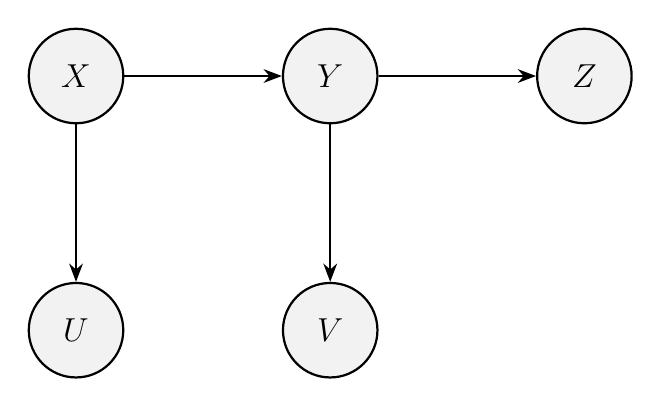
\begin{tikzpicture}[
    node distance=2cm and 2cm,
    every node/.style={circle, draw=black, fill=gray!10, minimum size=1.2cm, font=\large, align=center},
    every path/.style={thick, -{Stealth}}
]

% Nodes
\node (X) {$X$};
\node (Y) [right=of X] {$Y$};
\node (Z) [right=of Y] {$Z$};
\node (U) [below=of X] {$U$};
\node (V) [below=of Y] {$V$};

% Arrows
\draw (X) -- (Y);
\draw (Y) -- (Z);
\draw (X) -- (U);
\draw (Y) -- (V);

\end{tikzpicture}
\end{center}

\subsubsection{Question 1}
This question relates to the combinatorial (optimization) problem of finding all topological orderings of a given directed acyclic graph (DAG) with N vertices.

\begin{enumerate}[label=(\alph*)]
    \item What is the worst-case size of the configuration space $X$ for this combinatorial problem, in terms of $N$? Justify your answer. \hfill [2 marks]\\
    {\color{red}
    The worst case is $N!$}

    \item A DAG with no edges is said to be disconnected. Assume the DAG in Figure 1 is disconnected. How many possible topological orderings of the nodes are there? Justify your solution. \hfill [3 marks]\\
    {\color{red} $N!$}
    \item You must solve the problem of devising an efficient algorithm for computing all topological orderings of the DAG in Figure 1.
    \begin{enumerate}[label=(\roman*)]
        \item Give the steps in an exhaustive SDP algorithm for solving this problem. \hfill [5 marks]
        \item Use this SDP algorithm to compute the set of all possible topological orderings of this DAG. \hfill [6 marks]
    \end{enumerate}

    \item Now, assume the DAG in Figure 1 represents a probabilistic graphical model (PGM) over the random variables $X, Y, Z, U$ and $V$.
    \begin{enumerate}[label=(\roman*)]
        \item Using the topological ordering $[X, U, Y, V, Z]$ give the corresponding chain factorization of the joint distribution $P(X, Y, Z, U, V)$. \hfill [2 marks]\\
        \[
        P(X,U,Y,V,Z) = P(X)P(U|X)P(Y|X,U)P(V|X,U,Y)P(Z|X,U,Y,V)
        \]
        \item Using your chain factorization in (d)(i) above, remove all redundant dependencies from the conditional distributions, to give the Markov factorization of the joint distribution. \hfill [2 marks]
        \[
        P(X,U,Y,V,Z) = P(X)P(U|X)P(Y|X)P(V|Y)P(Z|Y)
        \]
    \end{enumerate}
\end{enumerate}

\usetikzlibrary{arrows.meta, positioning, shapes.multipart}
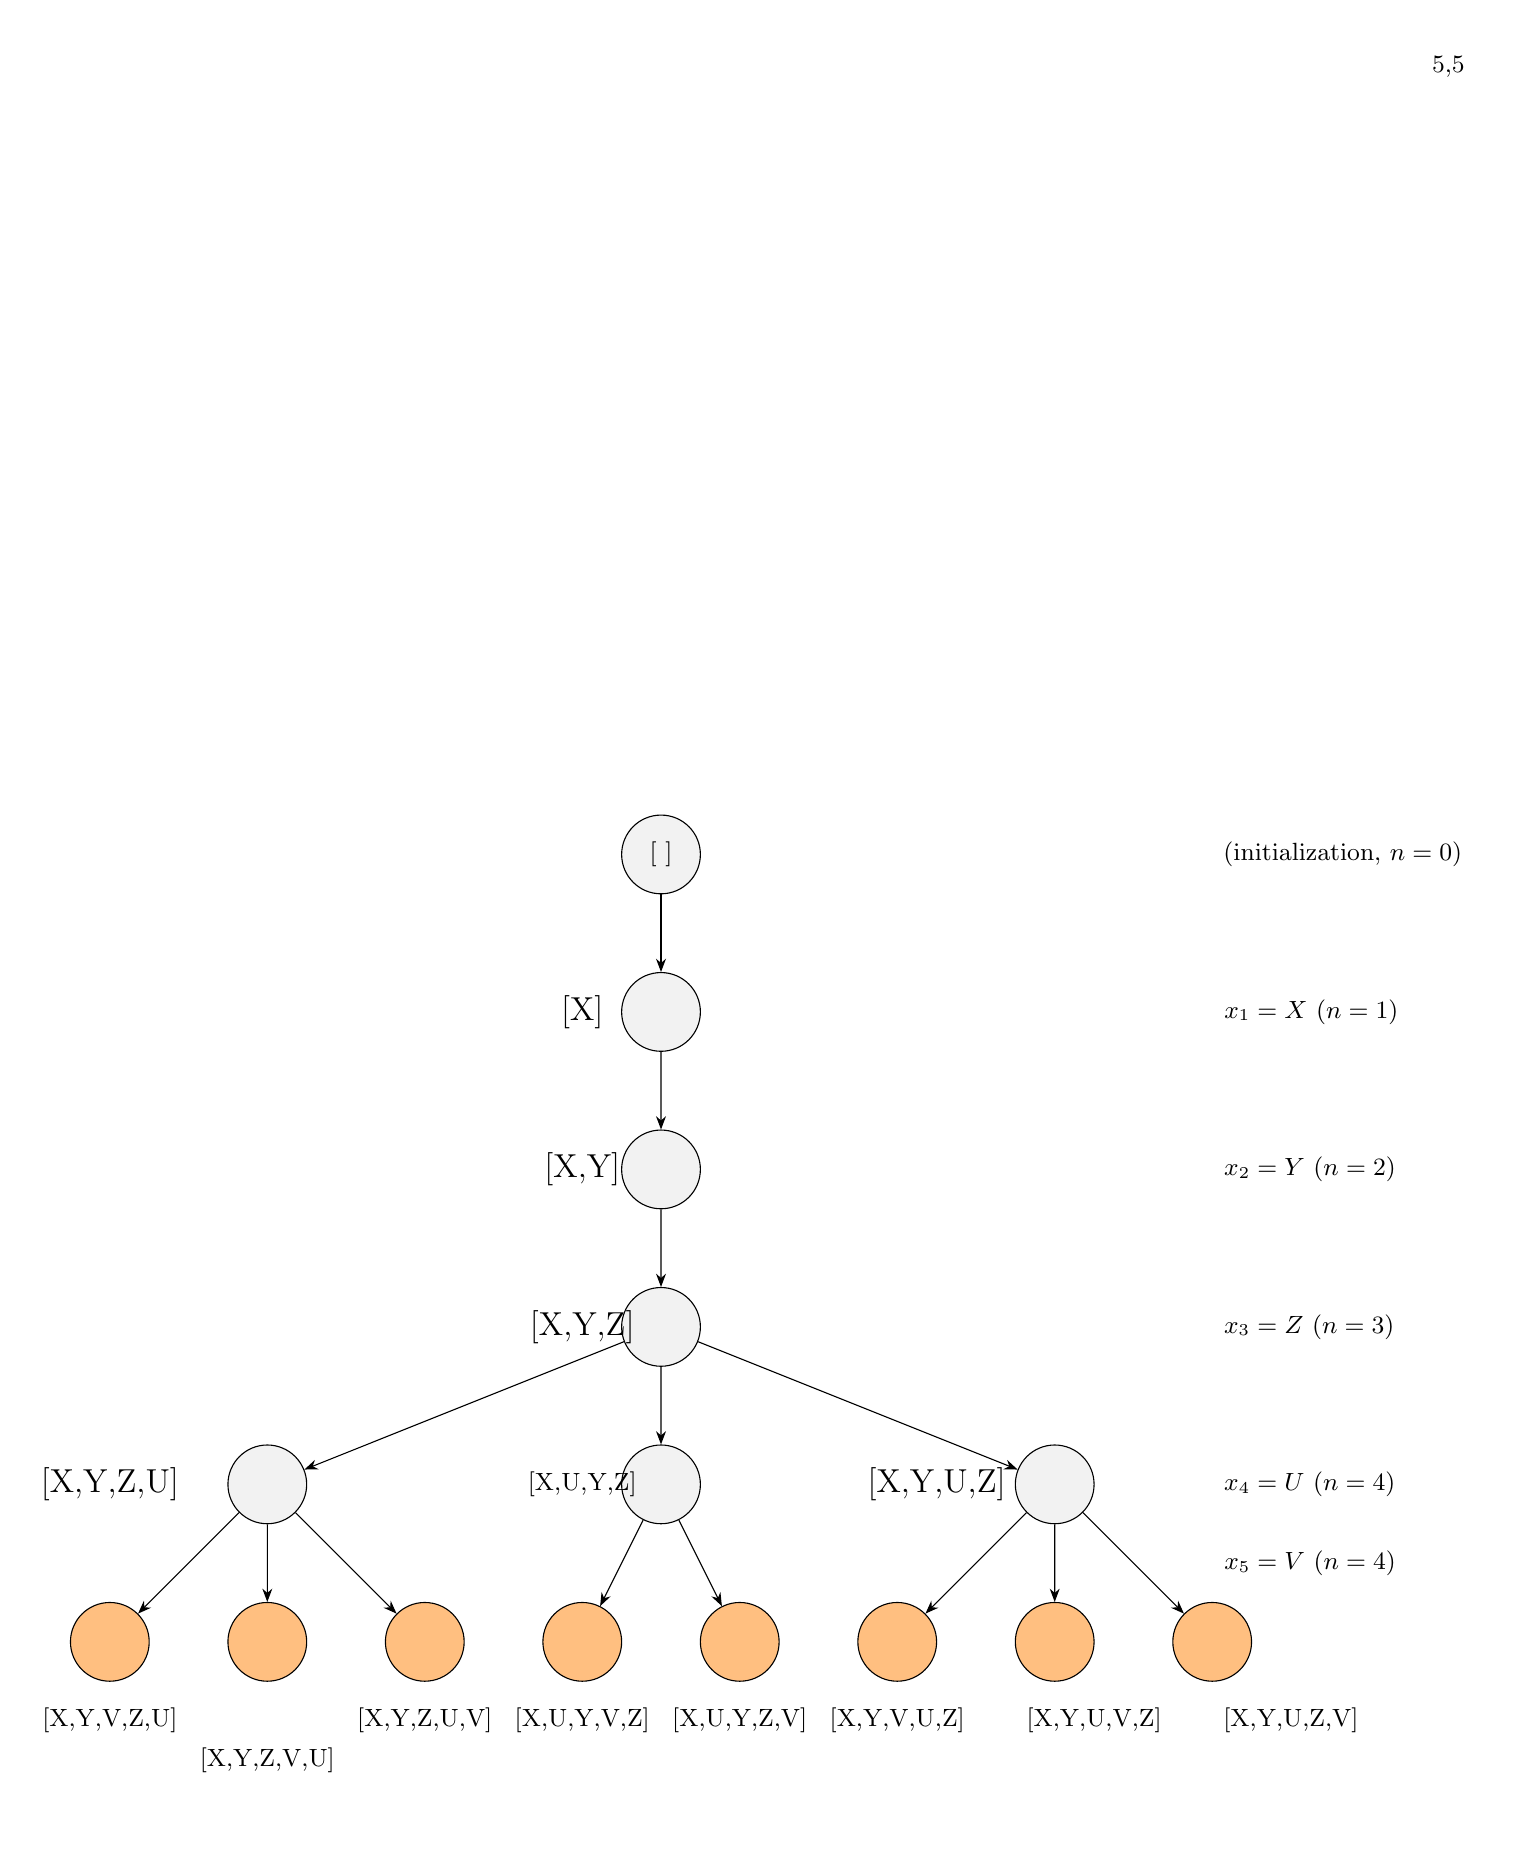
\begin{tikzpicture}[
  level distance=2cm,
  sibling distance=2.8cm,
  every node/.style={circle, draw, fill=gray!10, minimum size=1cm, font=\small},
  result node/.style={circle, draw, fill=orange!50, font=\small},
  edge from parent/.style={draw, -{Stealth}},
  level 4/.style={sibling distance=5cm},
  level 5/.style={sibling distance=2cm}
]

% Root and first level
\node {[\ ]}
  child {node {}
    child {node {}
      child {node {}
        % child {node[fill=orange!70] {[X,Y,Z,U]}}
        child {node {}
          child {node[result node] {}}
          child {node[result node] {}}
          child {node[result node] {}}
        }
        child {node {}
          child {node[result node] {}}
          child {node[result node] {}}
        }
        child {node {}
          child {node[result node] {}}
          child {node[result node] {}}
          child {node[result node] {}}
        }
      }
    }
  };
% Edge weights as raw text (not using node)
% \draw (0,0)  node[draw=none, fill=none, text=blue] {\small 0,0};
% \draw (-10,-10)  node[draw=none, fill=none, text=blue] {\small -5,-5};
\draw (10,10)  node[draw=none, fill=none] {\small 5,5};
\draw (-1,-2)  node[draw=none, fill=none] {\large [X]};
\draw (-1,-4)  node[draw=none, fill=none] {\large [X,Y]};
\draw (-1,-6) node[draw=none, fill=none] {\large[X,Y,Z]};
\draw (-7,-8)  node[draw=none, fill=none] {\large [X,Y,Z,U]};
\draw (-7,-11)  node[draw=none, fill=none] {\small [X,Y,V,Z,U]};
\draw (-5,-11.5)  node[draw=none, fill=none] {\small [X,Y,Z,V,U]};
\draw (-3,-11)  node[draw=none, fill=none] {\small [X,Y,Z,U,V]};

\draw (-1,-8)  node[draw=none, fill=none] {\small [X,U,Y,Z]};
\draw (-1,-11)  node[draw=none, fill=none] {\small [X,U,Y,V,Z]};
\draw (1,-11)  node[draw=none, fill=none] {\small [X,U,Y,Z,V]};

\draw (3.5,-8)  node[draw=none, fill=none] {\large [X,Y,U,Z]};
\draw (3,-11)  node[draw=none, fill=none] {\small [X,Y,V,U,Z]};
\draw (5.5,-11)  node[draw=none, fill=none] {\small [X,Y,U,V,Z]};
\draw (8,-11)  node[draw=none, fill=none] {\small [X,Y,U,Z,V]};
% Labels for n levels
\node[anchor=west,draw=none,fill=none] at (7,0) {(initialization, $n=0$)};
\node[anchor=west,draw=none,fill=none] at (7,-2) {$x_1 = X\ (n=1)$};
\node[anchor=west,draw=none,fill=none] at (7,-4) {$x_2 = Y\ (n=2)$};
\node[anchor=west,draw=none,fill=none] at (7,-6) {$x_3 = Z\ (n=3)$};
\node[anchor=west,draw=none,fill=none] at (7,-8) {$x_4 = U\ (n=4)$};
\node[anchor=west,draw=none,fill=none] at (7,-9) {$x_5 = V\ (n=4)$};

\end{tikzpicture}

\newpage
\subsubsection{Question 2}

\begin{center}
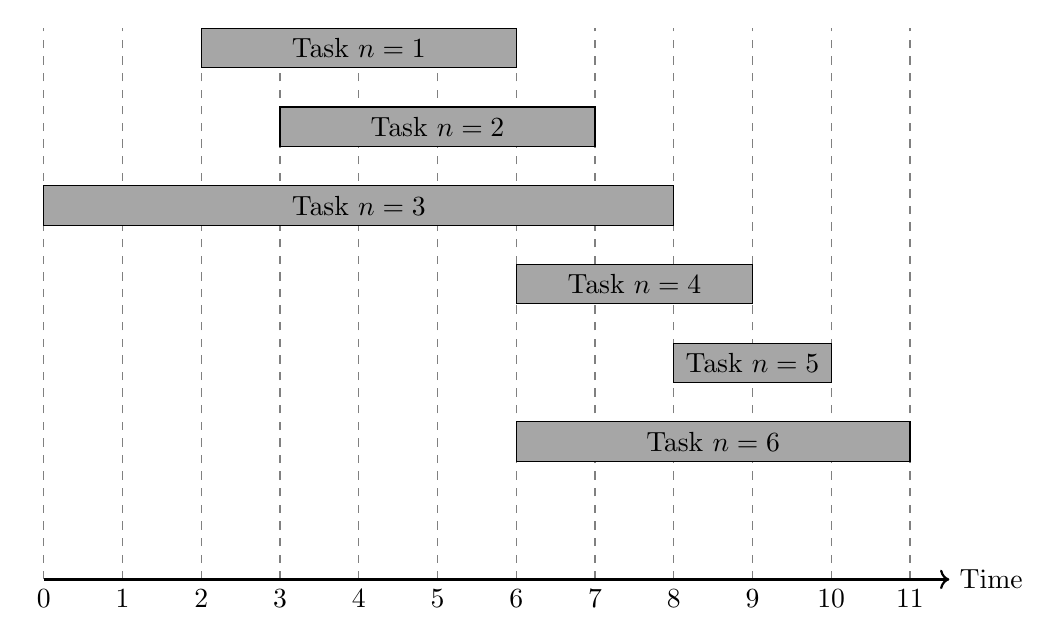
\begin{tikzpicture}
% Vertical grid lines
\foreach \x in {0,1,...,11} {
    \draw[dashed,gray] (\x,0) -- (\x,7);
    \node[below] at (\x,0) {\x};
}
% Time axis arrow
\draw[->,thick] (0,0) -- (11.5,0) node[right]{Time};

% Tasks (as bars): (start, y, length)
\draw[fill=gray!70] (2,6.5) rectangle (6,7) node[pos=.5] {Task $n=1$};
\draw[fill=gray!70] (3,5.5) rectangle (7,6) node[pos=.5] {Task $n=2$};
\draw[fill=gray!70] (0,4.5) rectangle (8,5) node[pos=.5] {Task $n=3$};
\draw[fill=gray!70] (6,3.5) rectangle (9,4) node[pos=.5] {Task $n=4$};
\draw[fill=gray!70] (8,2.5) rectangle (10,3) node[pos=.5] {Task $n=5$};
\draw[fill=gray!70] (6,1.5) rectangle (11,2) node[pos=.5] {Task $n=6$};
\end{tikzpicture}
\end{center}

\begin{enumerate}[label=(\alph*)]
    \item This question relates to dynamic programming as a method for combinatorial optimization.
    \begin{enumerate}[label=(\roman*)]
        \item Explain the principle of optimality. \hfill [2 marks]
        \item Explain how the principle of optimality reduces the computational complexity of an exact algorithm for solving an optimization problem. \hfill [3 marks]
        \item Explain the concept of memoization. \hfill [3 marks]
    \end{enumerate}

    \item Consider the planning problem of automatically selecting the best subset of a set of tasks to complete. Each of the $N = 6$ tasks is associated with a value, from the list $v = [20, 7, 4, 3, 10, 8]$. The optimal subset has the largest sum of values. Each task begins and ends at the times given in the schedule chart above. Tasks can only be selected together if they do not overlap. The list $p = [0, 0, 0, 1, 3, 1]$ gives the largest task index $n' < n$ such that task $n'$ does not overlap with task $n$.

    \begin{enumerate}[label=(\roman*)]
        \item Use the following Bellman recursion to compute the total value of the optimal subset of tasks, $V^\star_6$: \hfill [8 marks]
        \[
        V^\star_0 = 0
        \]
        \[
        V^\star_n = \max\left( V^\star_{n-1}, V^\star_{p_n} + v_n \right)
        \]

        {\color{blue}
        \begin{math}
        V^\star_0 = 0  \\
        V^\star_1 = \max\left(V^\star_0, V^\star_{p_1} + v_1 \right) = \max\left(0,0 + 20\right) = 20\\
        V^\star_2 = \max\left(V^\star_1, V^\star_{p_2} + v_2 \right) = \max\left(20,0 + 7\right) = 20 \\ 
        V^\star_3 = \max\left(V^\star_2, V^\star_{p_3} + v_3 \right) = \max\left(20,0 + 4\right) = 20 \\ 
        V^\star_4 = \max\left(V^\star_3, V^\star_{1} + v_4 \right) = \max\left(20,20 + 3\right) = 23 \\ 
        V^\star_5 = \max\left(V^\star_4, V^\star_{3} + v_5 \right) = \max\left(23,20 + 10\right) = 30 \\ 
        V^\star_6 = \max\left(V^\star_5, V^\star_{1} + v_6 \right) = \max\left(30,20 + 8\right) = 30 \\ 
        \end{math} 

        }
        \item What is the time complexity of this recursion? Justify your answer. \hfill [2 marks] \\
        {\color{blue}
        Given using memorization, the complexity is $O_{(n)}$
        }
        \item What is the worst-case time complexity of the exhaustive solution to this problem in general (that is, independent of the specific task values and start/end times)? Justify your answer. \hfill [2 marks]
    \end{enumerate}
\end{enumerate}

% \begin{tikzpicture}[
%   node distance=1.5cm and 2.5cm,
%   every node/.style={circle, draw=gray, fill=gray!10, minimum size=7mm},
%   level 1/.style={sibling distance=35mm},
%   level distance=1.5cm,
%   edge from parent/.style={draw, -{Stealth[length=2mm]}},
%   nonterminal/.style={draw=gray, fill=gray!10},
%   txt/.style={draw=none, fill=none, anchor=west}
% ]
% % Initialization node
% \node[nonterminal, label=right:{\small (initialization, $n=0$)}] (n0) at (0,0) {\small []};

% % Level 1
% \node[nonterminal] (n1a) at (0,-2) {\small [(0)]};
% \node[rectangle] (n1b) at (3,-2) {\small $P_1(20)$};
% \draw[->] (n0) -- (n1b);

% % Level 2
% \node[nonterminal] (n2a) at (0,-4) {\small []};
% \node[rectangle] (n2b) at (3,-4) {\small $P_2(17)$};
% \draw[->] (n1a) -- (n2b);

% % Level 3
% \node[nonterminal] (n3a) at (0,-6) {\small []};
% \node[rectangle] (n3b) at (3,-6) {\small $P_3(4)$};
% \draw[->] (n2a) -- (n3b);
% % Level 4
% \node[nonterminal] (n4a) at (0,-8) {\small []};
% \node[rectangle] (n4b) at (3,-8) {\small $V_4(3) + P_1(20)$};
% \draw[->] (n3a) -- (n4b);

% % Dashed horizontal lines
% \foreach \i in {1,2,3,4,5} {
%   \draw[dashed, gray] (-1.5,-2*\i) -- (10,-2*\i);
% }

% % Right-side labels
% \node[txt] at (10,-2) {$P1 = 20 (n=1)$};
% \node[txt] at (10,-4) {$P2 = 17 (n=2)$};
% \node[txt] at (10,-6) {$P3 = 4 (n=3)$};
% \node[txt] at (10,-8) {$P4 =  (n=4)$};

% \end{tikzpicture}

\pagebreak
\subsubsection{Question 3}

\begin{multicols}{2}
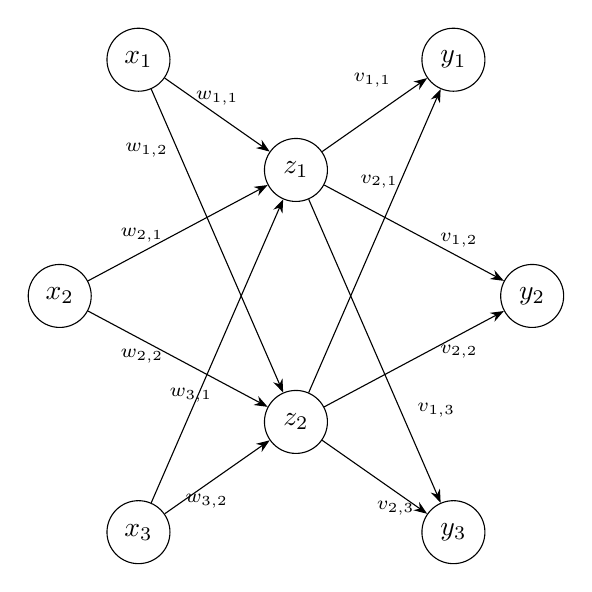
\begin{tikzpicture}[
  node distance=0.8cm and 1.5cm,
  neuron/.style={circle, draw=black, minimum size=8mm},
  ->, >=Stealth
]

% Inputs
\node[neuron] (x1) at (1,3) {$x_1$};
\node[neuron] (x2) at (0,0) {$x_2$};
\node[neuron] (x3) at (1,-3) {$x_3$};

% Hidden layer 1
\node[neuron] (z1) at (3,1.6) {$z_1$};
\node[neuron] (z2) at (3,-1.6) {$z_2$};

% Output layer
\node[neuron] (y1) at (5,3) {$y_1$};
\node[neuron] (y2) at (6,0) {$y_2$};
\node[neuron] (y3) at (5,-3) {$y_3$};

% Connections: Input to Hidden
\draw (x1) -- node[above] {\scriptsize $w_{1,1}$} (z1);
\draw (x1) -- node[pos=0.2,left] {\scriptsize $w_{1,2}$} (z2);
\draw (x2) -- node[pos=0.3,above] {\scriptsize $w_{2,1}$} (z1);
\draw (x2) -- node[pos=0.3,below] {\scriptsize $w_{2,2}$} (z2);
\draw (x3) -- node[pos=0.3,above] {\scriptsize $w_{3,1}$} (z1);
\draw (x3) -- node[pos=0.4,below] {\scriptsize $w_{3,2}$} (z2);

% Connections: Hidden to Output
\draw (z1) -- node[near end,above left] {\scriptsize $v_{1,1}$} (y1);
\draw (z1) -- node[near end,above] {\scriptsize $v_{1,2}$} (y2);
\draw (z1) -- node[near end,above right] {\scriptsize $v_{1,3}$} (y3);

\draw (z2) -- node[near end,below left] {\scriptsize $v_{2,1}$} (y1);
\draw (z2) -- node[near end,below] {\scriptsize $v_{2,2}$} (y2);
\draw (z2) -- node[pos=0.7,below] {\scriptsize $v_{2,3}$} (y3);
\end{tikzpicture}

\columnbreak
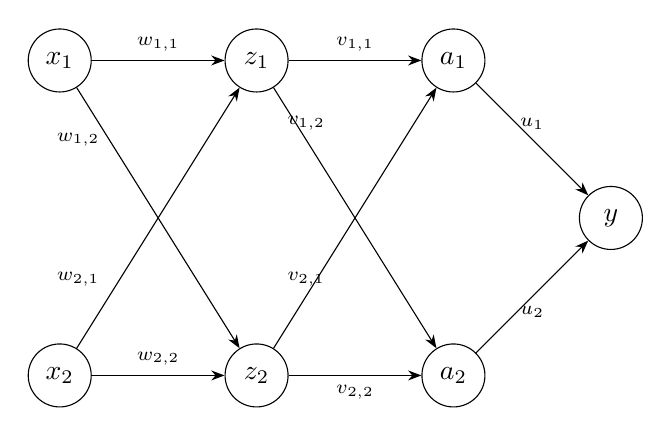
\begin{tikzpicture}[
  node distance=0.8cm and 1.5cm,
  neuron/.style={circle, draw=black, minimum size=8mm},
  ->, >=Stealth
]

% Inputs
\node[neuron] (x1) at (0,2) {$x_1$};
\node[neuron] (x2) at (0,-2) {$x_2$};

% Hidden layer 1
\node[neuron] (z1) at (2.5,2) {$z_1$};
\node[neuron] (z2) at (2.5,-2) {$z_2$};

% Hidden layer 2
\node[neuron] (a1) at (5,2) {$a_1$};
\node[neuron] (a2) at (5,-2) {$a_2$};

% Output
\node[neuron] (y) at (7,-0) {$y$};

% Connections: Input to Hidden 1
\draw (x1) -- node[pos=0.5,above] {\scriptsize $w_{1,1}$} (z1);
\draw (x1) -- node[pos=0.2,left] {\scriptsize $w_{1,2}$} (z2);

\draw (x2) -- node[pos=0.2,above left] {\scriptsize $w_{2,1}$} (z1);
\draw (x2) -- node[pos=0.5,above] {\scriptsize $w_{2,2}$} (z2);
% Connections: Hidden 1 to Hidden 2
\draw (z1) -- node[above] {\scriptsize $v_{1,1}$} (a1);
\draw (z1) -- node[pos=0.2,above] {\scriptsize $v_{1,2}$} (a2);

\draw (z2) -- node[pos=0.2,above] {\scriptsize $v_{2,1}$} (a1);
\draw (z2) -- node[below] {\scriptsize $v_{2,2}$} (a2);
% Connections: Hidden 2 to Output
\draw (a1) -- node[above] {\scriptsize $u_1$} (y);
\draw (a2) -- node[below] {\scriptsize $u_2$} (y);
\end{tikzpicture}
\end{multicols}{2}



\begin{enumerate}[label=(\alph*)]
    \item For the deep neural network of Figure 2(a) (autoencoder) above with softplus activation nonlinearities, write down the formulae for the hidden nodes $z_1, z_2$ and the output nodes $y_1, y_2, y_3$. \hfill [6 marks]

    \item The formulae for the deep network of Figure 2(b) are given in matrix form as:
    \[
    z = \max(0, W^T x), \quad a = \max(0, V^T z), \quad y = \max(0, U^T a)
    \]
    with weights
    \[
    W = \begin{bmatrix}
    0.1 & 0.7 \\
    -0.3 & 0.2
    \end{bmatrix}, \quad
    V = \begin{bmatrix}
    1.3 & -0.5 \\
    0.3 & -1.4
    \end{bmatrix}, \quad
    U = \begin{bmatrix}
    0.6 \\
    -0.1
    \end{bmatrix}
    \]

    \begin{enumerate}[label=(\roman*)]
        \item For inputs with value $x = [3 \quad 2]^T$, compute the values of the first hidden layer $z$. \hfill [4 marks] \\
        {\color{blue}
        \begin{math}
         z_1 = \max \left(0,x_1 w_{1,1} + x_2 w_{2,1} \right) \\ 
             = \max \left(0,3 \times 0.1 + 2 \times (-0.3) \right) \\
             = 0 \\
         z_2 = \max \left(0,x_1 w_{1,2} + x_2 w_{2,2} \right)  \\
            = \max \left(0,3 \times 0.7 + 2 \times 0.2  \right) \\
            = 2.5 \\
        \end{math}
        }
        \item Given that the values of the second hidden layer are $a = [0.75 \quad 0]^T$, compute the value of the output $y$. \hfill [4 marks] \\

    \end{enumerate}

    \item Using dual numbers for automatic differentiation, derive two dual number formulae: one for $y$ paired with $y_{u1}$ (its derivative with respect to the weight $u_1$) and the other for $y$ paired with $y_{u2}$ (derivative with respect to weight $u_2$). Both expressions should be in terms of the hidden outputs $a$ and parameters $U$. Show your working. \hfill [6 marks]
\end{enumerate}
